\section{\LARGE{Trasformazione delle cellule di eschericchia coli xl1 blue}}

\vspace{0.6cm}


\subsection{Sommario}

\subsubsection{Scopo}


L'obbiettivo di questa esperienza è quello di manipolare le \textbf{culture batteriche di E.coli} (batterio gram negativo non patogeno usato comunenmente all'nterno dei laboratori di ricerca), andando a \textbf{trasportare il plasmide pUC18}, precedentemente trattato, all'interno di questi batteri per poi andare ad essere quello che è un ceppo di propagazione(atto al clonaggio e alla propagazione di plasmidi) all'interno di un terreno di crescita.


\subsubsection{Cenni teorici}


Il procedimento di trasporto del dsDNA da esterno alla cellula all'interno è chiamato \textbf{trasformazione batterica}, ed è un fenomeno parasessuale che consente ai batteri lo scambio di materiale genico.


Solo alcune specie batteriche possono acquisire DNA estraneo dall'ambiente (DNA esogeno) che deve essere a doppia elica con facilità, queste sono dette cellule \textit{"naturalmente competenti"}, altre specie invece diventano competenti solo in particolari condizioni fisiologiche ed altre ancora come per esempio E.coli  necessitano di una trasformazione artificiale in laboratorio tramite vari metodi chimici o fisici (da noi usato è il metodo dello \textit{shock-termico} ) che le rende \textbf{competenti}.


una volta che il plasmide si trova all'interno della cellula batterica di E.coli, questa la si fa crescere all'interno di piastre precedentemente preparate con LB-agar-amp (Luria Bertani medium with ampicillin), in grado di fornire il nutrimento necessario alla cellula per potersi nutrire e clonare, producendo molte cellule batteriche contenenti molti plasmidi ingegnerizzati di nostro interesse.

 
\subsection{Materiali utilizzati}

\begin{itemize}
	\item Guanti in lattice 
	\item Provette Eppendorf (2mL)
	\item Micropipette (100-1000  e 2-200 microlitri  )
	\item Scatola di polistirolo contenente ghiaccio
	\item Bagno termostatico
	\item piasra di LB-agar-amp
	\item bacchette in vetro 
\end{itemize}


\subsection{Soluzioni utilizate}

\begin{itemize}

	\item miniprep del pUC18
	\item cellule competenti 
	\item LB liquido 

\end{itemize}



\subsection{Procedimento}

\begin{enumerate}

	\item Come primo lavoro si è dovuto diluire la nostra miniprep del pUC18 (descritta nell'esperienza numero 1) in acqua pura in misura 1:10 quindi, necessitando ai passi successivi di 1 microlitro di soluzione diluita, si è ritenuto adeguato prelevare 1 microlitro  di miniprep del pUC18 e 9 microlitri  di acqua pura tramite una micropipetta e inserire le due componenti in una nuova provetta eppendorf da 2 mL.
	
	
	\item Si è andati ora a lavorare in una \textit{ambiente biologicamente sterile} per poter prelevare sotto cappa biologica 100 microlitri  di cellule competenti, e li si è messi in una provetta eppendorf sempre da 2 mL.  Lavorando in un ambiente sterile si garantisce che il nostro ambiente sia protetto da agenti inquinanti derivanti dall’esterno.
	
	\item A questo punto all'interno della eppendorf contenente le cellule competenti si è andato ad aggiungere 1  microlitro della miniprep, diluita con acqua al passo n° 1, così formando una soluzione contenente sia le cellule batteriche che i plasmidi che dovranno poi entrare all'interno delle cellule. 
	
	\item Una volta che la soluzione è stata Agitata per far si che i plasmidi si distribuiscano in modo unitario all'interno della soluzione, si va ad incubare la provetta contenente la soluzione in ghiaccio, una trentina di minuti per far si che la temperatura si abbassi gradualmente di qualche grado e che i plasmidi si vadano a legare sulla membrana della cellula batterica.
	
	\item Passata una mezz'ora, la temperatura della soluzione contenente cellule e plasmidi si è raffreddata e stabilizzata ad una bassa temperatura e in linea teorica i plasmidi si sono ancorati alle membrane delle cellule dove dovranno poi essere incorporati, ora bisogna effettuare un'operazione di cruciale importanza, cioè lo  \textbf{shock termico}, portando la provetta eppendorf da una temperatura di ca. 0°C(ghiaccio) ad una temperatura di 42°C  molto rapidamente e lasciarla nel bagno termostatico per 1 minuto (il tempo è importante poichè se si lascia il tutto ad una temperatura alta per troppo tempo le cellule batteriche potrebbero morire).  Questo passaggio fa si che all'interno delle cellule batteriche di E.coli si \textit{aprano dei pori}, in grado di far passare il DNA esogeno nella parte interna della membrana, cioè all'interno della cellula formando così una  \textbf{cellula trasformata}, al cui interno c'è il plasmide contenente il gene interessato. 
	(un'altro metodo per poter effettuare l'apertura dei pori e la sucessiva immissione dei plasmidi all'interno delle cellule competenti è l'elettroporazione che consiste in una repentina scarica elettrica ad alto voltaggio, il vantaggio di qeusta è che può essere applicata anche a cellule eucariotiche)
	
	\begin{figure}[H]
	
		\centering
		\subfloat{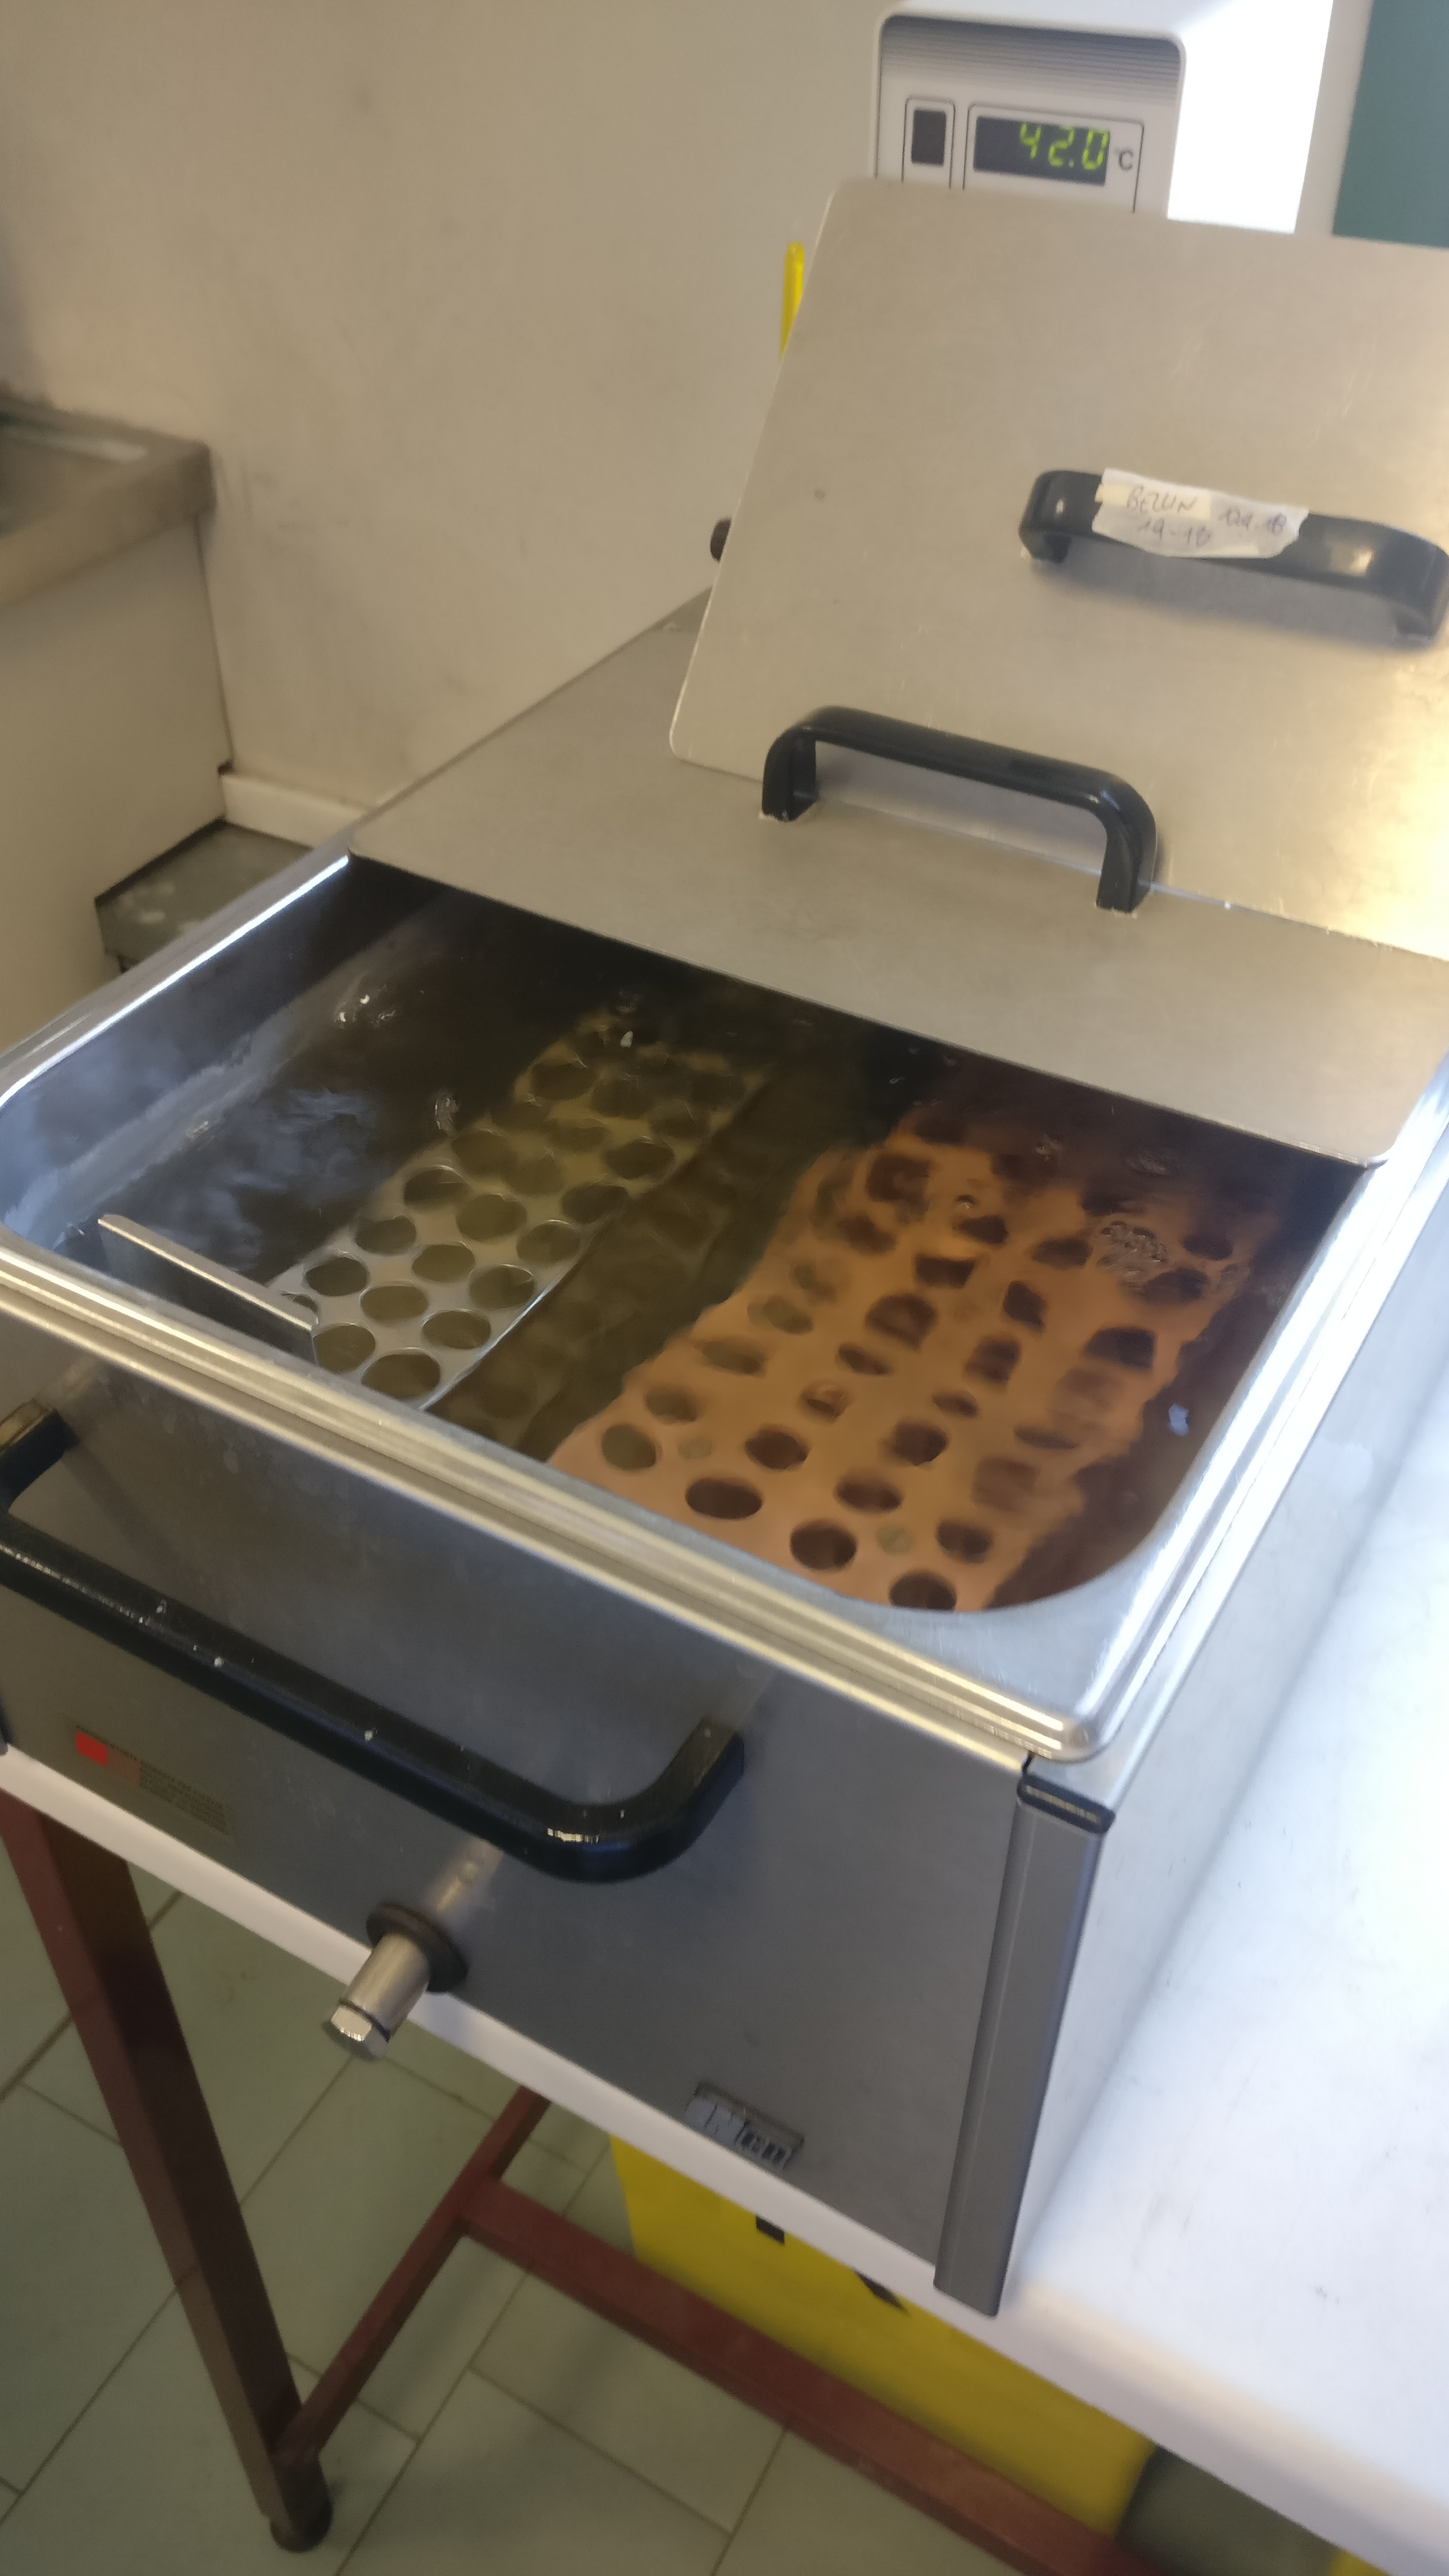
\includegraphics[width=0.3\textwidth]{./immagini/bagno_termostatico.jpg}} \quad
		\subfloat{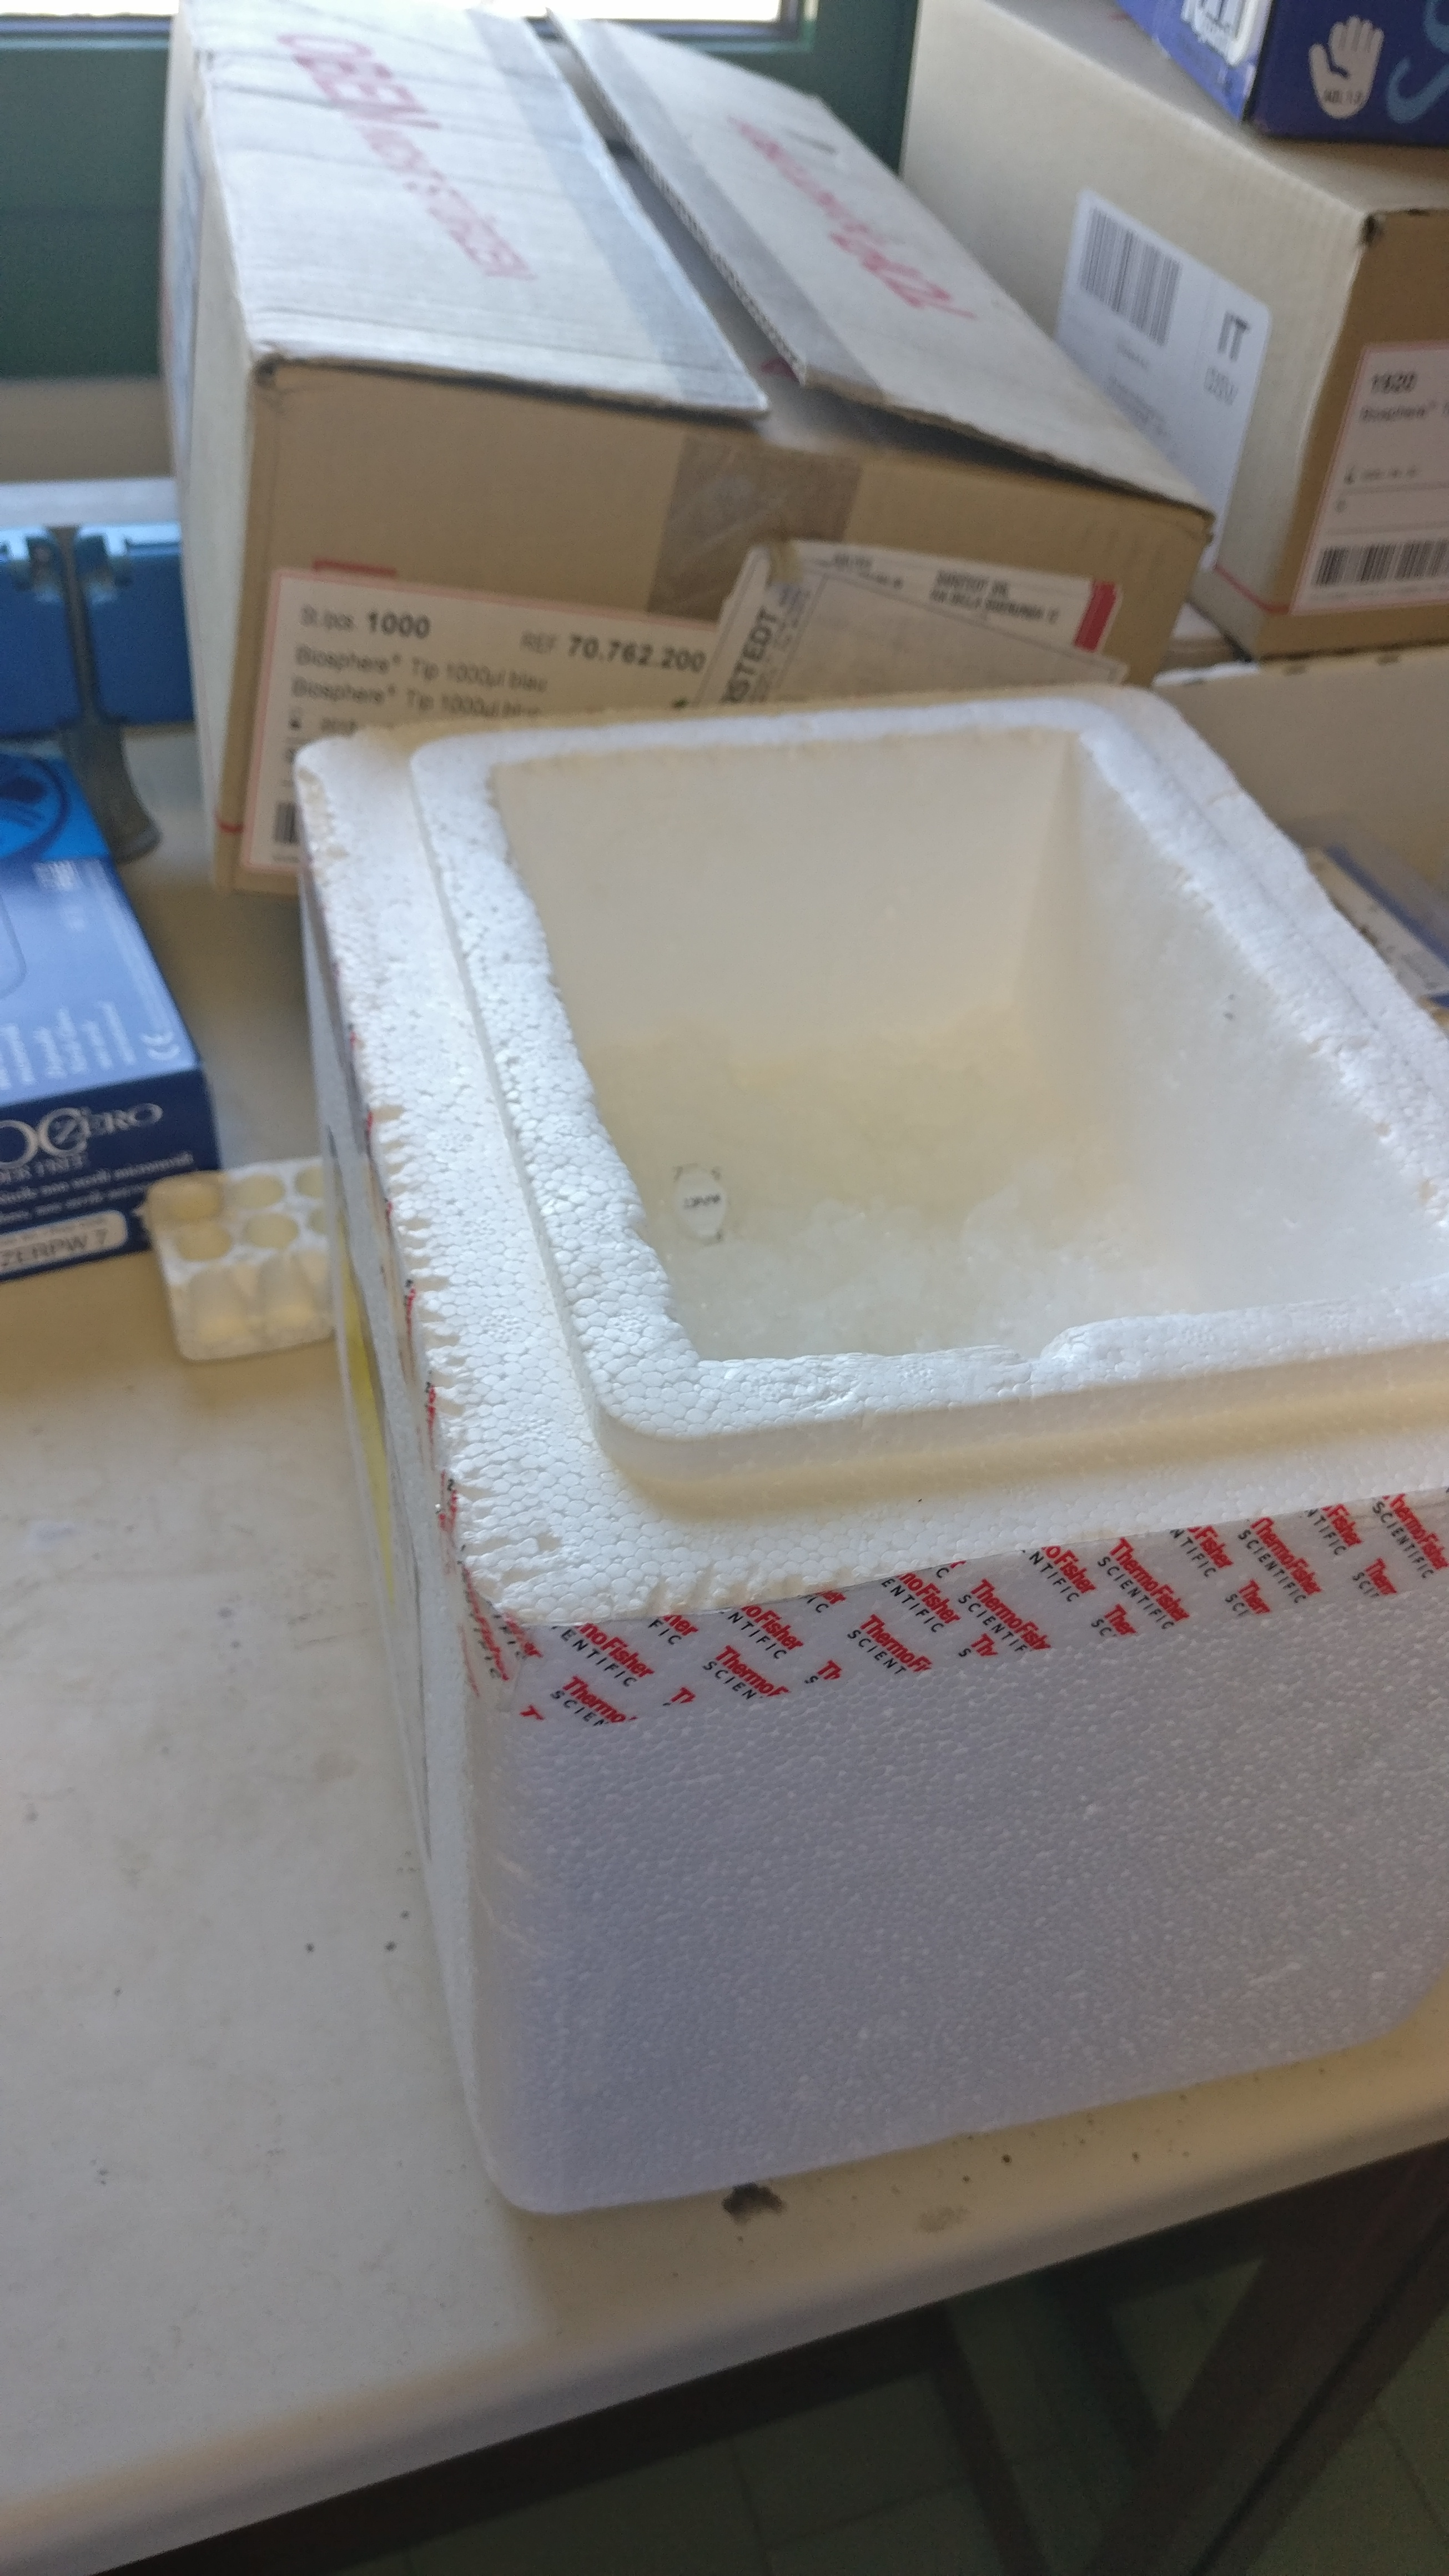
\includegraphics[width=0.3\textwidth]{./immagini/ghiaccio.jpg}}
		\caption{Bagno termostatico e immersione in ghiaccio}
		\label{bango_e_ghiaccio}
	
	
	\end{figure}
	
	\item Subito passato il minuto si prende di nuovo la eppendorf e la si rimette in ghiaccio per altri 5 minuti, facendo in questo modo si favorisce di nuovo il \textit{rallentamento del metabolismo cellulare}. 
	
	\item Si aggiunge poi del nutriente LB liquido all'interno della provetta, e la si incuba a 37°C per 1 ora, facendo così, la cultura batterica si accresce e si esprime la  \textbf{resistenza all'antibiotico} (ampicillina) (gene contenuto all'interno del plasmide) per poter poi sapere, una volta messo sul terreno di LB-amp se il nostro plasmide è stato effettivamente incorporato all'interno della cellula batterica o no.
	
	\vspace{0.3cm}
	
	
	\begin{figure}[H]
		
		\centering
		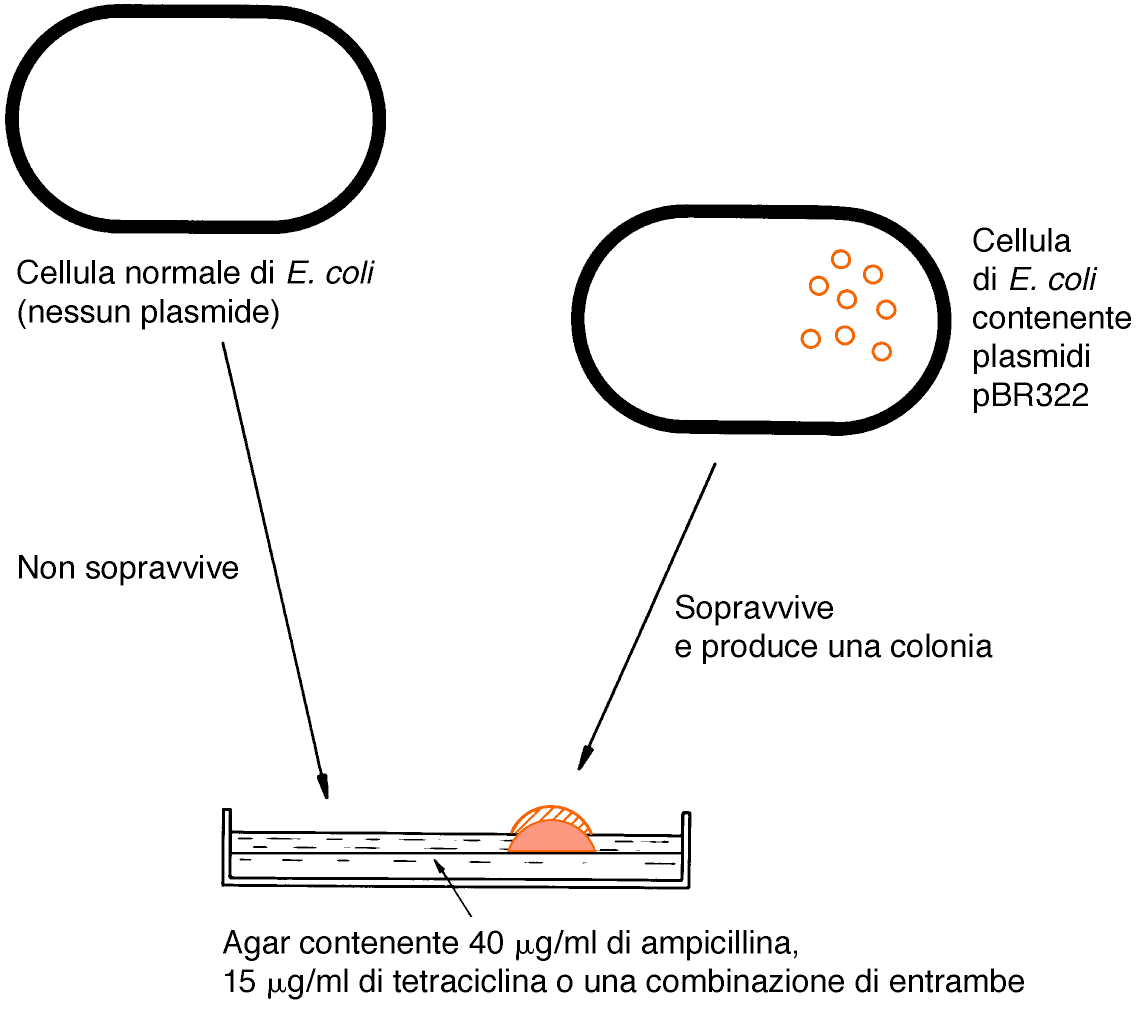
\includegraphics[width=0.6\textwidth]{./immagini/resistenza_ampicillina.png}
		\caption{Colonie con il plasmide integrato resistono al terreno con ampicillina }
		\label{resistenza ampicillina}
	
	\end{figure}
	
	\item Come ultimo passaggio si va a piastrare 150-200 microlitri  della sospensione delle cellule precedentemente incubate a 37°C, su di una piastra di LB-amp, distribuendole con una bacchetta di vetro a forma di 'L' su tutta la superficie della piastra, le si mettono poi ad una temperatura di 37°C per una notte a crescere.    
	
	\begin{figure}[H]
	
		\centering
		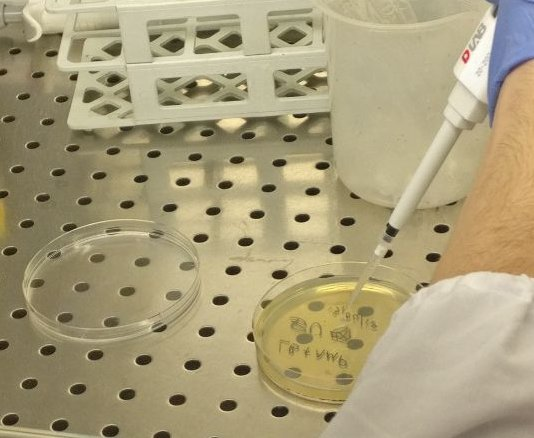
\includegraphics[width=0.6\textwidth]{./immagini/piastraggio_colonie.jpg}
		\caption{Piastraggio delle cellule di E. Coli su terreno LB-Amp}
		\label{piastraggio cellule}
	
	\end{figure}



\end{enumerate}


\subsection{Risultati e Conclusioni}

Tramite questa Procedura si è potuto inserire all'interno delle nostre cellule batteriche di E.coli rese competenti, i plasmidi pUC18 contenenti i geni di mio interesse da clonare, o da esprimere. 
